%Chapter 2
\chapter{Overview of simulation and compressed air applications}
\thispagestyle{empty}
\vspace{38em}
\hrulefill
\\
\enquote*{\textit{Quote.}} - Somebody\\
\clearpage
\section{Introduction}
\section{Review of compressed air energy interventions in industry}
	\subsection{Preamble}
		Compressed air improvement can be obtained through intervention in either the supply or demand of compressed air \cite{Kriel2014Masters}. Improvements in supply interventions are achieved by increasing the efficiency of compressed air supply. Examples of this type of intervention include \gls{dcs}, compressor maintenance, etc. 
		\par
		Due to the size of mining compressed air networks, there is often a larger scope for improvement in air demand. Improving the  demand is achieved by optimising air flow consumers, reducing leaks, etc.
		\par
	 	From literature, this section will review compressed air energy interventions that have performed in industry.
	 	
	\subsection{Strategies to improve compressed air supply}
	
		\subsubsection{Optimising compressor control}
		Compressors types and numbers can differ widely from mining compressed air systems. Compressor selection is crucial in these systems to match the correct compressors with the requirements of the system. \cite{marais2010expert}
		- Setpoints\\
		- schecdules
		- Variable speed drives\\
		
		\subsubsection{Dynamic compressor selection}
		
		\subsubsection{Reconfiguring compressed air networks}
			A number of old mining compressed air systems  have not been adequately maintained and improved. Often they cannot sufficiently supply air to meet the demand or air is provided from non optimal sources. In a study by Bredenkamp \cite{Bredenkamp2013Masters}, reconfiguring of the air network was investigated to improve these systems.
			\par  
			In the study, Bredenkamp investigated interconnecting the compressed air systems of two mining shafts and relocating of a compressor. This strategy lead to an average power reduction of 1.7 MW and an estimated annual energy cost saving of R8.9M at the time.
			\par 
			\textit{Discussion of Bredenkamp}
			
	\subsection{Strategies to reduce compressed air demand}
	As illustrated in \cref{fig: Mining schedule}
		- Reducing leaks\\
		- 
		- Marais PhD\\
		- Snyman - investigated various Compressed air demand reduction and efficiency
		 optimisations \cite{Snyman2011Masters}.
		 
		 \subsubsection{Leakage detection}
		 Air leaks are a major inefficiency in mining compressed air systems. Improving leaks is relatively easier method to  reduce air demand and improve the efficiency of the system is to remove leaks in the system \cite{van2011sustaining}. Air leaks occur as a result of open pipes, fissure and breaks. Losses depend on the size of the leak. Figure \real{} shows the expected energy lossed vs leakage area. *** Still gotta make figure ***
		 \par
		 
		 A number of techniques are utilised in industry to identify cair leaks.- Pascoe [38]
		 A simple method to reduce air demand and improve the efficiency of the system is to remove leaks in the network. n oder
		 (Van Tonder masters)
		 - Inspections\\
		 - Audible sounds (by ear)\\
		 - Ultrasonic\\
		 - Intelligent leakage detection (instrumentaion SCADA)\\
		 - Alternatives (pigging, soap water, Dyes load/unload test)\\
		 -  CALDS ( Compressed air leakage document system)et al investigated increased energy savings through the use of \gls{calds} \cite{marais2009increased}.	
		 
		 \subsection{Underground control valves}
		 - Pascoe
		 
		\subsubsection{Improving pneumatic rock drills efficiency}
		 Pneumatic rock drills are on of the largest air consumers in a mine. Improving the efficiency or drilling can have a significant energy impact of the system. In a study by  Bester \textit{et al.} \cite{bester2013effect} looking at the effect of compressed air pressure on energy demand. Bester showed that between 2002 and 2013 compressed air and energy consumption per tonne of ore produced had steadily increased. This is illustrated  in \cref{fig: Compressed energy and air flow per ton}. 
		 \par 
		 The increase of air consumption per \gls{t} was a result of reduced air pressure at the mining areas. This causes the drilling rate to drop leading to higher air consumption. Pressure measurements as low as 300 \gls{kpa} were recorded in these areas. Before 2002 the drilling pressure at the mining section (stopes), was maintained above 500 \gls{kpa} at most mines. 
		 \par 
		 \begin{figure}[h]
		 	\centering
		 	% GNUPLOT: LaTeX picture with Postscript
\begingroup
  \makeatletter
  \providecommand\color[2][]{%
    \GenericError{(gnuplot) \space\space\space\@spaces}{%
      Package color not loaded in conjunction with
      terminal option `colourtext'%
    }{See the gnuplot documentation for explanation.%
    }{Either use 'blacktext' in gnuplot or load the package
      color.sty in LaTeX.}%
    \renewcommand\color[2][]{}%
  }%
  \providecommand\includegraphics[2][]{%
    \GenericError{(gnuplot) \space\space\space\@spaces}{%
      Package graphicx or graphics not loaded%
    }{See the gnuplot documentation for explanation.%
    }{The gnuplot epslatex terminal needs graphicx.sty or graphics.sty.}%
    \renewcommand\includegraphics[2][]{}%
  }%
  \providecommand\rotatebox[2]{#2}%
  \@ifundefined{ifGPcolor}{%
    \newif\ifGPcolor
    \GPcolortrue
  }{}%
  \@ifundefined{ifGPblacktext}{%
    \newif\ifGPblacktext
    \GPblacktextfalse
  }{}%
  % define a \g@addto@macro without @ in the name:
  \let\gplgaddtomacro\g@addto@macro
  % define empty templates for all commands taking text:
  \gdef\gplbacktext{}%
  \gdef\gplfronttext{}%
  \makeatother
  \ifGPblacktext
    % no textcolor at all
    \def\colorrgb#1{}%
    \def\colorgray#1{}%
  \else
    % gray or color?
    \ifGPcolor
      \def\colorrgb#1{\color[rgb]{#1}}%
      \def\colorgray#1{\color[gray]{#1}}%
      \expandafter\def\csname LTw\endcsname{\color{white}}%
      \expandafter\def\csname LTb\endcsname{\color{black}}%
      \expandafter\def\csname LTa\endcsname{\color{black}}%
      \expandafter\def\csname LT0\endcsname{\color[rgb]{1,0,0}}%
      \expandafter\def\csname LT1\endcsname{\color[rgb]{0,1,0}}%
      \expandafter\def\csname LT2\endcsname{\color[rgb]{0,0,1}}%
      \expandafter\def\csname LT3\endcsname{\color[rgb]{1,0,1}}%
      \expandafter\def\csname LT4\endcsname{\color[rgb]{0,1,1}}%
      \expandafter\def\csname LT5\endcsname{\color[rgb]{1,1,0}}%
      \expandafter\def\csname LT6\endcsname{\color[rgb]{0,0,0}}%
      \expandafter\def\csname LT7\endcsname{\color[rgb]{1,0.3,0}}%
      \expandafter\def\csname LT8\endcsname{\color[rgb]{0.5,0.5,0.5}}%
    \else
      % gray
      \def\colorrgb#1{\color{black}}%
      \def\colorgray#1{\color[gray]{#1}}%
      \expandafter\def\csname LTw\endcsname{\color{white}}%
      \expandafter\def\csname LTb\endcsname{\color{black}}%
      \expandafter\def\csname LTa\endcsname{\color{black}}%
      \expandafter\def\csname LT0\endcsname{\color{black}}%
      \expandafter\def\csname LT1\endcsname{\color{black}}%
      \expandafter\def\csname LT2\endcsname{\color{black}}%
      \expandafter\def\csname LT3\endcsname{\color{black}}%
      \expandafter\def\csname LT4\endcsname{\color{black}}%
      \expandafter\def\csname LT5\endcsname{\color{black}}%
      \expandafter\def\csname LT6\endcsname{\color{black}}%
      \expandafter\def\csname LT7\endcsname{\color{black}}%
      \expandafter\def\csname LT8\endcsname{\color{black}}%
    \fi
  \fi
    \setlength{\unitlength}{0.0500bp}%
    \ifx\gptboxheight\undefined%
      \newlength{\gptboxheight}%
      \newlength{\gptboxwidth}%
      \newsavebox{\gptboxtext}%
    \fi%
    \setlength{\fboxrule}{0.5pt}%
    \setlength{\fboxsep}{1pt}%
\begin{picture}(9360.00,4032.00)%
    \gplgaddtomacro\gplbacktext{%
      \colorrgb{0.42,0.42,0.42}%
      \put(682,924){\makebox(0,0)[r]{\strut{}$0$}}%
      \colorrgb{0.42,0.42,0.42}%
      \put(682,1230){\makebox(0,0)[r]{\strut{}$5$}}%
      \colorrgb{0.42,0.42,0.42}%
      \put(682,1536){\makebox(0,0)[r]{\strut{}$10$}}%
      \colorrgb{0.42,0.42,0.42}%
      \put(682,1842){\makebox(0,0)[r]{\strut{}$15$}}%
      \colorrgb{0.42,0.42,0.42}%
      \put(682,2148){\makebox(0,0)[r]{\strut{}$20$}}%
      \colorrgb{0.42,0.42,0.42}%
      \put(682,2453){\makebox(0,0)[r]{\strut{}$25$}}%
      \colorrgb{0.42,0.42,0.42}%
      \put(682,2759){\makebox(0,0)[r]{\strut{}$30$}}%
      \colorrgb{0.42,0.42,0.42}%
      \put(682,3065){\makebox(0,0)[r]{\strut{}$35$}}%
      \colorrgb{0.42,0.42,0.42}%
      \put(682,3371){\makebox(0,0)[r]{\strut{}$40$}}%
      \colorrgb{0.42,0.42,0.42}%
      \put(814,704){\makebox(0,0){\strut{}$2002$}}%
      \colorrgb{0.42,0.42,0.42}%
      \put(2025,704){\makebox(0,0){\strut{}$2004$}}%
      \colorrgb{0.42,0.42,0.42}%
      \put(3237,704){\makebox(0,0){\strut{}$2006$}}%
      \colorrgb{0.42,0.42,0.42}%
      \put(4448,704){\makebox(0,0){\strut{}$2008$}}%
      \colorrgb{0.42,0.42,0.42}%
      \put(5659,704){\makebox(0,0){\strut{}$2010$}}%
      \colorrgb{0.42,0.42,0.42}%
      \put(6871,704){\makebox(0,0){\strut{}$2012$}}%
      \colorrgb{0.42,0.42,0.42}%
      \put(8082,704){\makebox(0,0){\strut{}$2014$}}%
      \colorrgb{0.42,0.42,0.42}%
      \put(8214,924){\makebox(0,0)[l]{\strut{}$0$}}%
      \colorrgb{0.42,0.42,0.42}%
      \put(8214,1230){\makebox(0,0)[l]{\strut{}$50$}}%
      \colorrgb{0.42,0.42,0.42}%
      \put(8214,1536){\makebox(0,0)[l]{\strut{}$100$}}%
      \colorrgb{0.42,0.42,0.42}%
      \put(8214,1842){\makebox(0,0)[l]{\strut{}$150$}}%
      \colorrgb{0.42,0.42,0.42}%
      \put(8214,2148){\makebox(0,0)[l]{\strut{}$200$}}%
      \colorrgb{0.42,0.42,0.42}%
      \put(8214,2453){\makebox(0,0)[l]{\strut{}$250$}}%
      \colorrgb{0.42,0.42,0.42}%
      \put(8214,2759){\makebox(0,0)[l]{\strut{}$300$}}%
      \colorrgb{0.42,0.42,0.42}%
      \put(8214,3065){\makebox(0,0)[l]{\strut{}$350$}}%
      \colorrgb{0.42,0.42,0.42}%
      \put(8214,3371){\makebox(0,0)[l]{\strut{}$400$}}%
    }%
    \gplgaddtomacro\gplfronttext{%
      \csname LTb\endcsname%
      \put(176,2147){\rotatebox{-270}{\makebox(0,0){\strut{}kWh/t}}}%
      \put(8851,2147){\rotatebox{-270}{\makebox(0,0){\strut{}$m^3$/t}}}%
      \put(4448,374){\makebox(0,0){\strut{}Year}}%
      \put(4448,3701){\makebox(0,0){\strut{}Compressed air energy and Volume consumed per ton}}%
      \csname LTb\endcsname%
      \put(3593,173){\makebox(0,0)[r]{\strut{}Energy per Ton (kWh/t)}}%
      \csname LTb\endcsname%
      \put(7352,173){\makebox(0,0)[r]{\strut{}Volume per Ton ($m^3$/t)}}%
    }%
    \gplbacktext
    \put(0,0){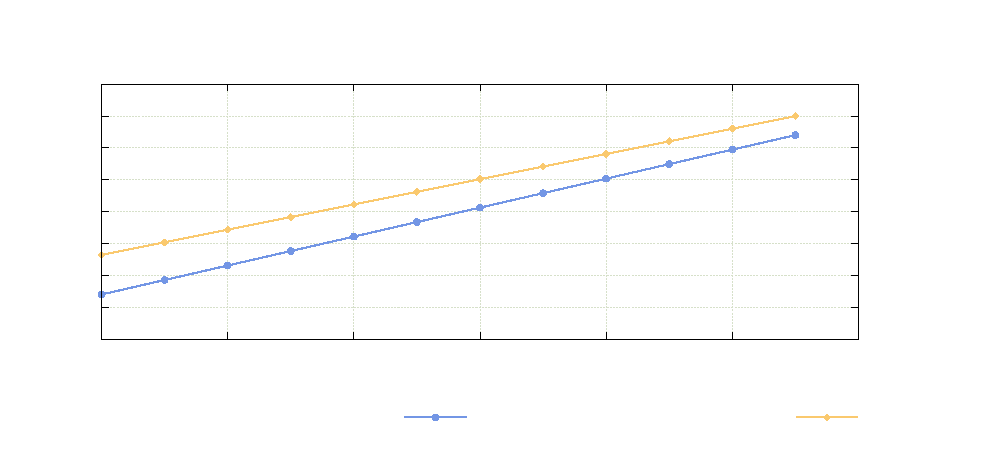
\includegraphics{Graphs/1/EVperT/EVperT}}%
    \gplfronttext
  \end{picture}%
\endgroup

		 	\caption[The Compressed air energy and flow consumed per T of ore produced.]{The Compressed air energy and flow consumed per T of ore produced. Adopted from Bester \textit{et al.} \cite{bester2013effect}.}
		 	\label{fig: Compressed energy and air flow per ton}
		 \end{figure}
		 From the literature, it is shown that lowering the pressure reduces the efficiency and drill rate of rock drilling, leading to higher air consumption. Interventions that reduce systemic air losses or optimise supply can increase the pressure operating pressure. Increased pressure, during the drilling shift, may add more value than the energy cost savings that can be achieved at a lower pressure.
	\subsection{Summary}
\clearpage

\section{Use of simulations to identify improvements in mining systems}
	\subsection{Preamble}
	\subsection{Simulation tools}
	\subsection{Value of simulation in DSM projects}
		(Van Niekerk M)\\
		- Compressed air \\
		- Cooling systems\\
		- Dewatering\\
		- Design optimisations using simulation\\
		- De Coning -  simulations to investigate the opportunity to optimise the control strategy of a compressed air network by rescheduling the compressors.
	\subsection{Simulation procedures}
	
		-Kriel masters\\
		 \glspl{vsd} (or \glspl{vfd}) \\
		-Pascoe
		\subsubsection{Periodic simulation}
 	\subsection{Verifying simulations}
 		- Holman
 		- van Niekerk masters\\
 		- Kriel masters ( validation)\\
 		- Calibrating -pascoe
 		- determining accuracy - pascoe
 		- Du2015Development
 		- comparisons with models
 		- comparison with actual 
 		- First principles
 	
	
	\section{Use of simulation in compressed air system optimisation}
	
	\subsection{Estimation techniques}
	- Snyman estimated improvements using historical data.\cite{Snyman2011Masters}\\
	- Marais estimation through simplified estimation, simulation \cite{Marais2012PhD, marais2013simplification}.
	\clearpage	
	
	\subsubsection{Shortcoming of previous studies}
		\label{Shortcomings of previous work}
	\subsection{Summary}
\section{Conclusion}